\documentclass{article}
\usepackage{float}

% Language setting
% Replace `english' with e.g. `spanish' to change the document language
\usepackage[english]{babel}

% Set page size and margins
% Replace `letterpaper' with`a4paper' for UK/EU standard size
\usepackage[letterpaper, top=1.5cm, bottom = 1.5cm, left = 1.5cm, right = 1.5cm, marginparwidth=1.75cm]{geometry}

% Useful packages
\usepackage{amsmath}
\usepackage{graphicx}
\usepackage[colorlinks=true, allcolors=blue]{hyperref}

\title{Exploring the relationship between climate attitudes and extreme weather events - S\&DS 625 Final Project}
\author{Megan Ayers}


\begin{document}
\maketitle

\section{Introduction}
\subsection{Contextualizing and motivating}
Climate change and environmental degradation is one of the most existential
crises of our time, if not the most existential. Unfortunately, many
Americans do not agree with this statement and/or do not fully comprehend the
implications of our global future if we do not address the causes of
climate change. Without recognition of the seriousness of climate change,
harmful consumer habits perpetuate, eco-friendly policies falter due to lack
of support, and the industries and corporations that negatively impact the
environment are not held accountable nor pressured to abandon the status-quo.
Climate communication is a field that works with these issues, and in
particular, with how to educate and persuade individuals about climate
change and the necessity of acting to reduce it. The hope is that
the more people there are that recognize climate change as a serious threat,
the more likely we are to have politicians and corporations that are
pressured to use their positions of power to enact positive change when it
comes to the environment. 

This contextualizes the goal for this final project - to better understand
some aspects of climate change beliefs at the county-level. If we don't 
understand the beliefs that people currently have about climate change,
and what factors might influence those beliefs, then we will be less
effective at trying to persuade those people than if we can be understanding
and empathetic at the same time as being convincing. In particular, this
report investigates how local extreme weather events relate to county-level
climate change beliefs. Perhaps personally experiencing one of
the widely broadcasted affects of climate change - increased extreme weather
events such as drought, hurricanes, wildfires, winter storms, etc - would
cause a person to take climate change more seriously, compared to someone
who just hears about these things happening on the news. However, there are
other cultural and demographic factors that are expected to have an effect
on climate change opinions that also need to be controlled for, such as
political leanings and age.


\subsection{Data sources}
To explore the relationship between extreme weather events and climate
change opinion with consideration given to the additional impact of
political leanings and demographics on climate change beliefs, the analysis
draws on information from multiple data sources. 

Data collected and processed by the Yale Program on Climate Change
Communication is used to understand climate change belief (the response
variable of this analysis). This data consists of US
county-level estimates of climate change beliefs, i.e. x\% of the population
in New Haven County believes that climate change is happening. These
estimates are calculated from a large-scale nation-wide survey ($n > 25,000$)
conducted in spring of 2020, and were "derived from a statistical model using
multilevel regression with post-stratification (MRP)". Though using
individual-level data could be more convincing for arguing existence of a
relationship between extreme weather event experiences and climate change
beliefs (the unit "county" does not itself have a climate change belief),
actually obtaining the supplementary data at this level was not feasible for
this project due to data privacy issues. 

Supplementary demographic data at the county level was collected from the Census
Bureau's ACS 2019 estimates using the R package `tidycensus`. To understand
the political leaning of each county, 2020 general election results were obtained
at the county level. These came from a data set containing general election
results from 2000-2020 maintained by the MIT Election Data and Science Lab
and accessed via the Harvard Dataverse. 

Identifying counties that experienced an extreme weather event around the
time of the climate opinion survey is not cut-and-dried. How should one
define "extreme weather"? There may be multiple reasonable responses
to this question, but this report defines "extreme weather" as
weather events that were declared disasters by FEMA
(Federal Emergency Management Agency). Records of these events from 1953 to
2021 are recorded in the online OpenFEMA Data Sets at the state and county level.
FEMA disasters were chosen as the indicator of extreme weather because
they signal a disaster beyond what state governments typically expect and are
prepared to handle. This accounts for the fact that independently of climate
change, some parts of the country naturally experience - and are used to
experiencing - more severe weather than others.


\section{Data Preparation}

Merging these data sources required cleaning and quality
assurance checks of each individual source.

\subsection{Climate change opinion survey data}
Because the providers of the climate change opinion survey already processed
the individual responses into county-level estimates, this data is very clean
to begin with. Data is available for every county reported on by the Census
in 2020, there are no duplicate rows, and the response variable `happening`
(indicating the proportion of county population that believes climate change
is happening) is relatively Normal in distribution. Note that the original
survey file contains data for many different climate-related questions asked
in the survey, but this analysis focuses only on the high level
question of existence of climate change.

\subsection{Election data}
This data set required a little more work to clean up. Data was reported for
one county that was not recognized as a county by the Census, and was dropped. For
some reason, San Joaquin County CA had missing data, which was found 
manually from the county website and replaced. Votes were sometimes
recorded by the mode in which they were received (ex. "Early Vote", 
"Absentee", "Election Day" etc.) and sometimes in total, so aggregation to 
the total county level had to be standardized between counties. All differences in county names between this source and the 
Census Bureau (which was regarded as ground truth for standardizing all sources
to use FIPS codes for future merging) could be rectified except for voting districts in Alaska.
I was unable to find a way to map voting districts to Census-reported
counties, so I dropped Alaska from the analysis. Although the other data
sources do have information on Alaska, political leaning was clearly such a
strong indicator of climate change belief that it seems preferable to
drop it entirely from the analysis rather than introduce missing values for
political leaning.
Figure 1 shows the geographic distribution of the county-level 2020 election
results, while also indicating whether that county has above or below average
belief in climate change (compared to the political group average, not the
overall average).

\subsection{Census demographic data}
The ACS 2019 estimates obtained through the Census were very clean and
required almost no cleaning aside from reshaping the data and renaming one
county to be consistent with a recent name change. The analysis begins with  
information about the gender, race, and ethnicity breakdowns of each county,
along with the median income and age of each county. Population
proportions are calculated for use in the analysis instead of the raw total counts.

\subsection{FEMA weather data}
Given the choice of the FEMA data set, there remains a tension between the
ideas that experiencing multiple events over a longer time scale would have
a larger impact on people's mindsets, but also that it is harder to safely
assume that the same individuals are remaining in the same county over a
longer time scale. In an attempt to balance these competing interests,
counties are flagged as "affected by extreme weather" if they experienced
a FEMA declared event in 2019 (the closest data to when the climate opinion
survey was collected), and also experienced at least 2 FEMA declared events
between 2015-2018. This second requirement is an attempt to capture counties
where extreme weather is more likely to be seen as recurrent rather than a
fluke. 511 (a little over 16\%) US counties meet this requirement. Note that
the original data sets include FEMA disasters that are non-weather related,
such as earthquakes, biological disasters, chemical disasters, terrorist
disasters, etc. This analysis considers hurricanes, floods, severe storms,
fires, snow, tornados, severe ice storms, coastal storms, typhoons, and
droughts. Figure 2 displays all FEMA declared weather disasters from 2015-2019,
as well as highlighting the counties which meet the requirements outlined above
to be considered as "affected by severe weather" in the analysis.

\begin{figure}[H]
\centering
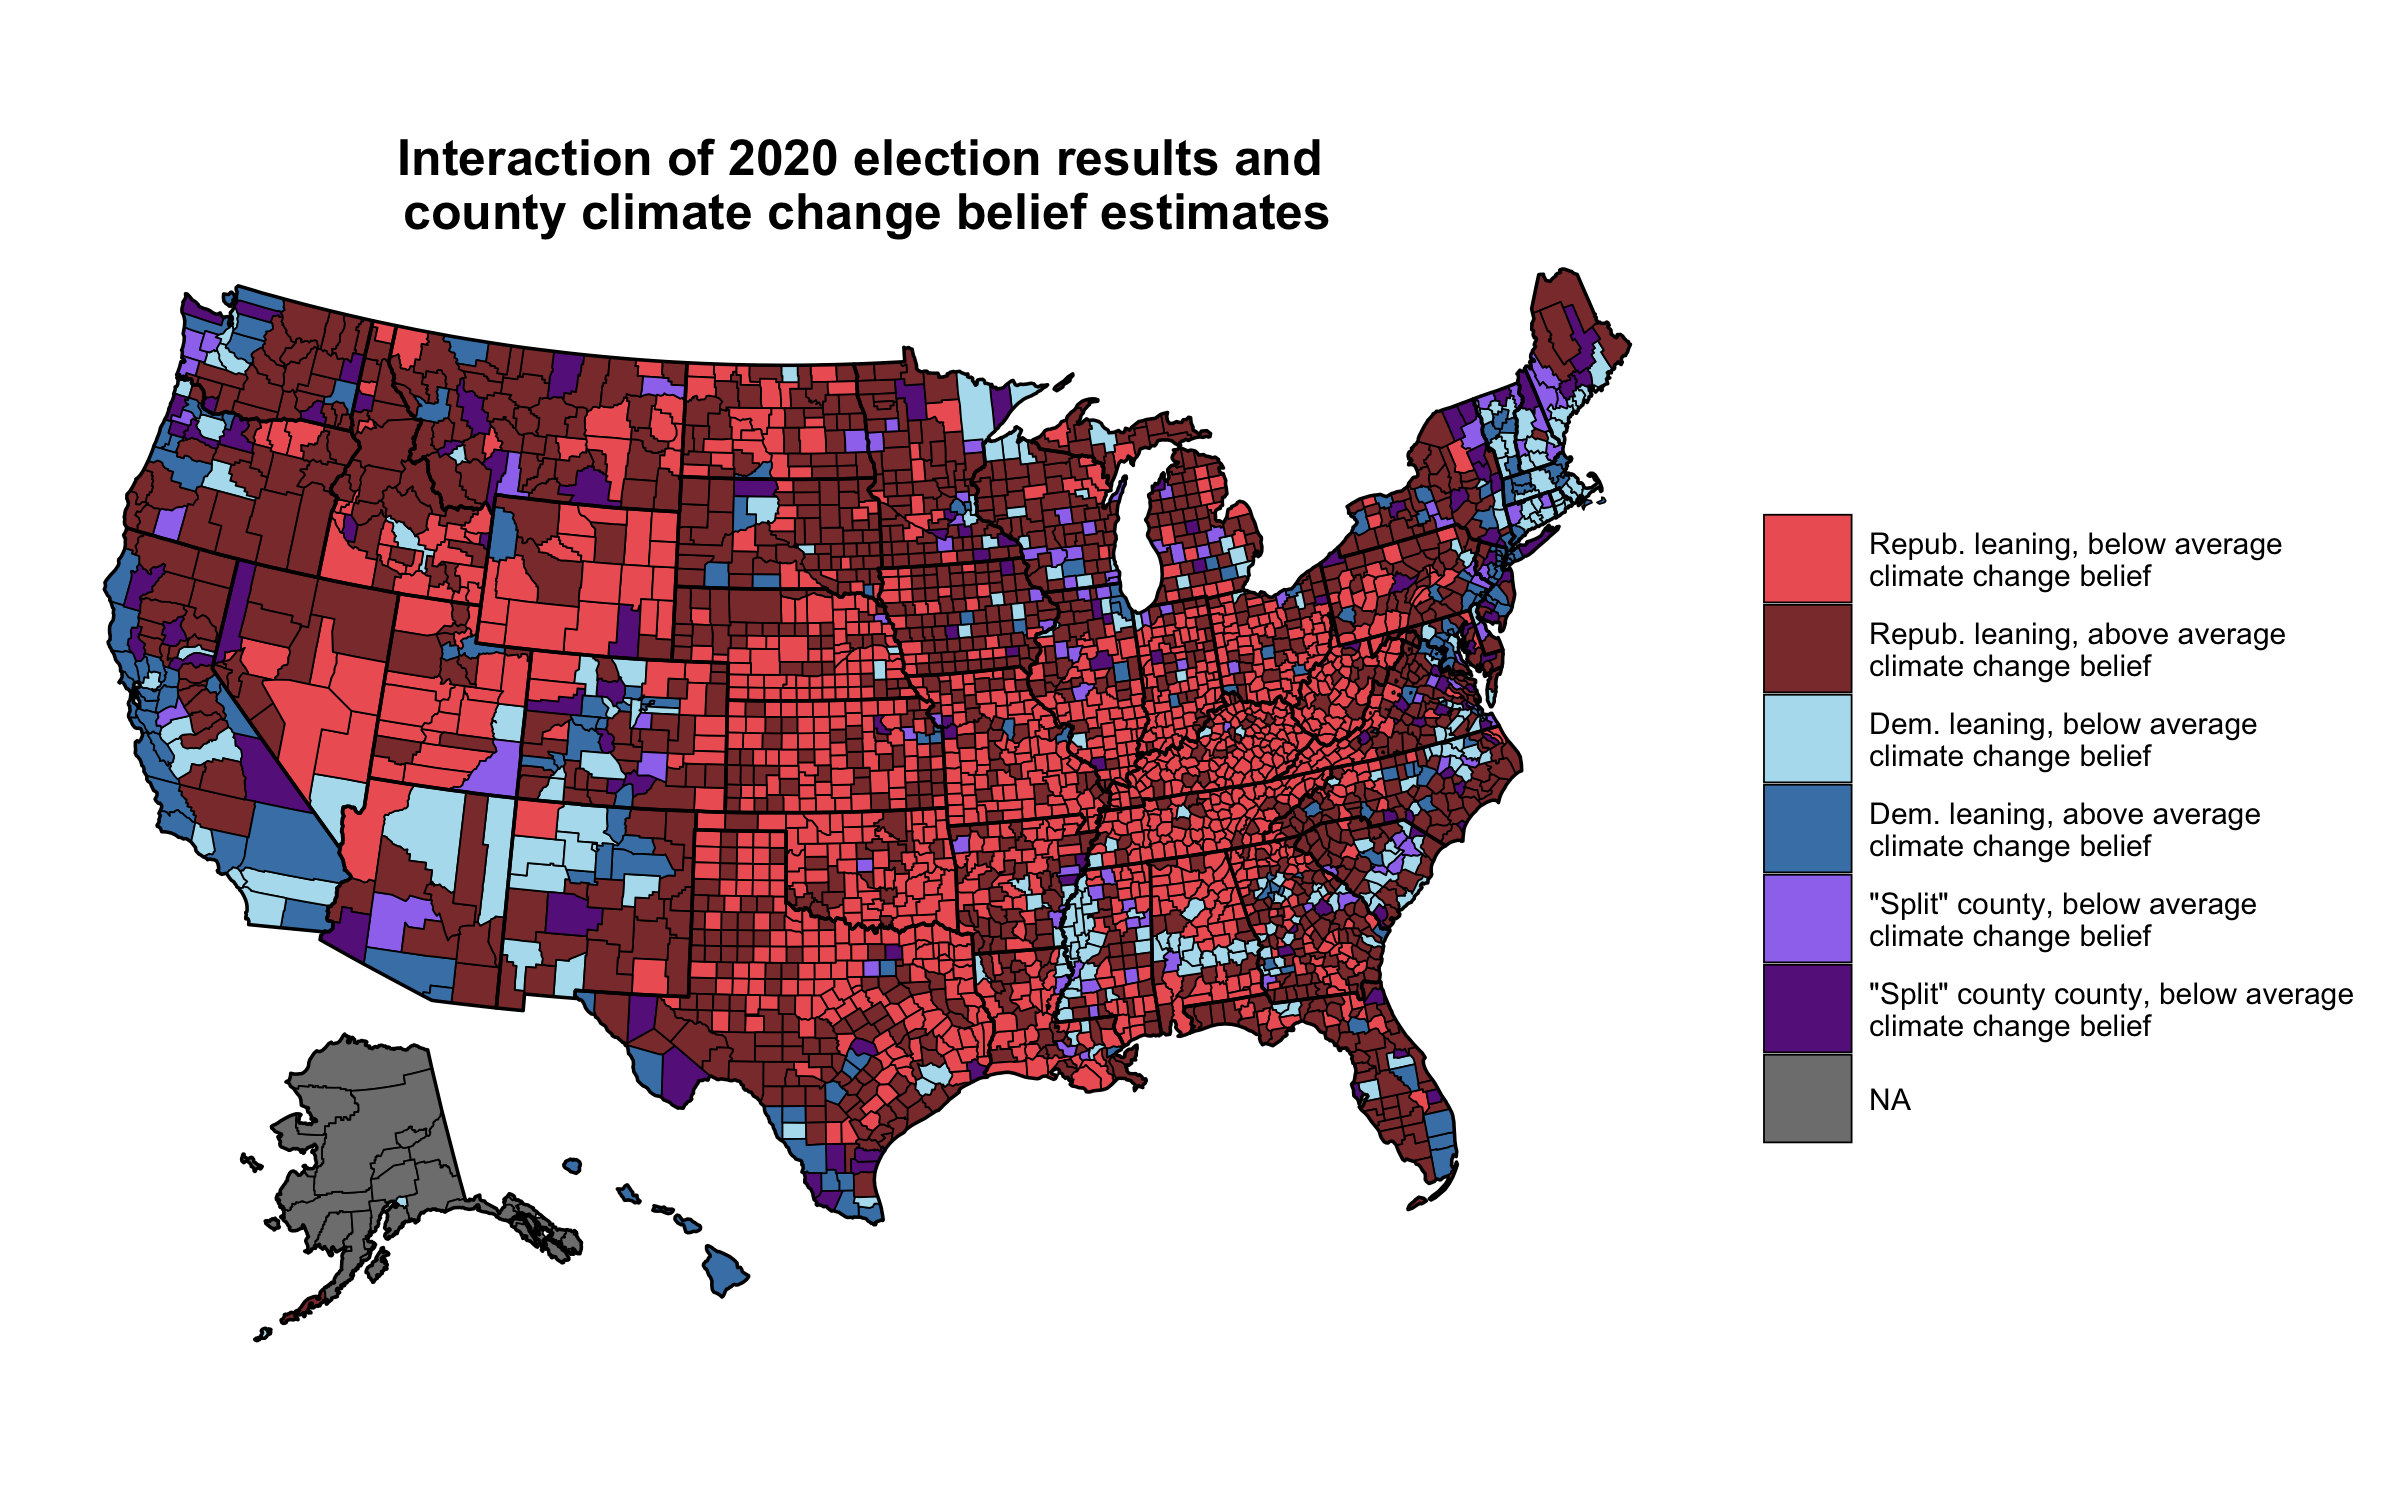
\includegraphics[scale=0.225]{images/election_climate_beliefs_map_in_group_comp.png}
\caption{This figure shows the 2020 presidential election results at the county level while also showing whether these counties have climate change belief above/below average compared to their political group. "Split" counties refers to counties where neither Democrats nor Republicans won more than 52.5\% of the vote.}
\end{figure}


\begin{figure}[H]
\centering
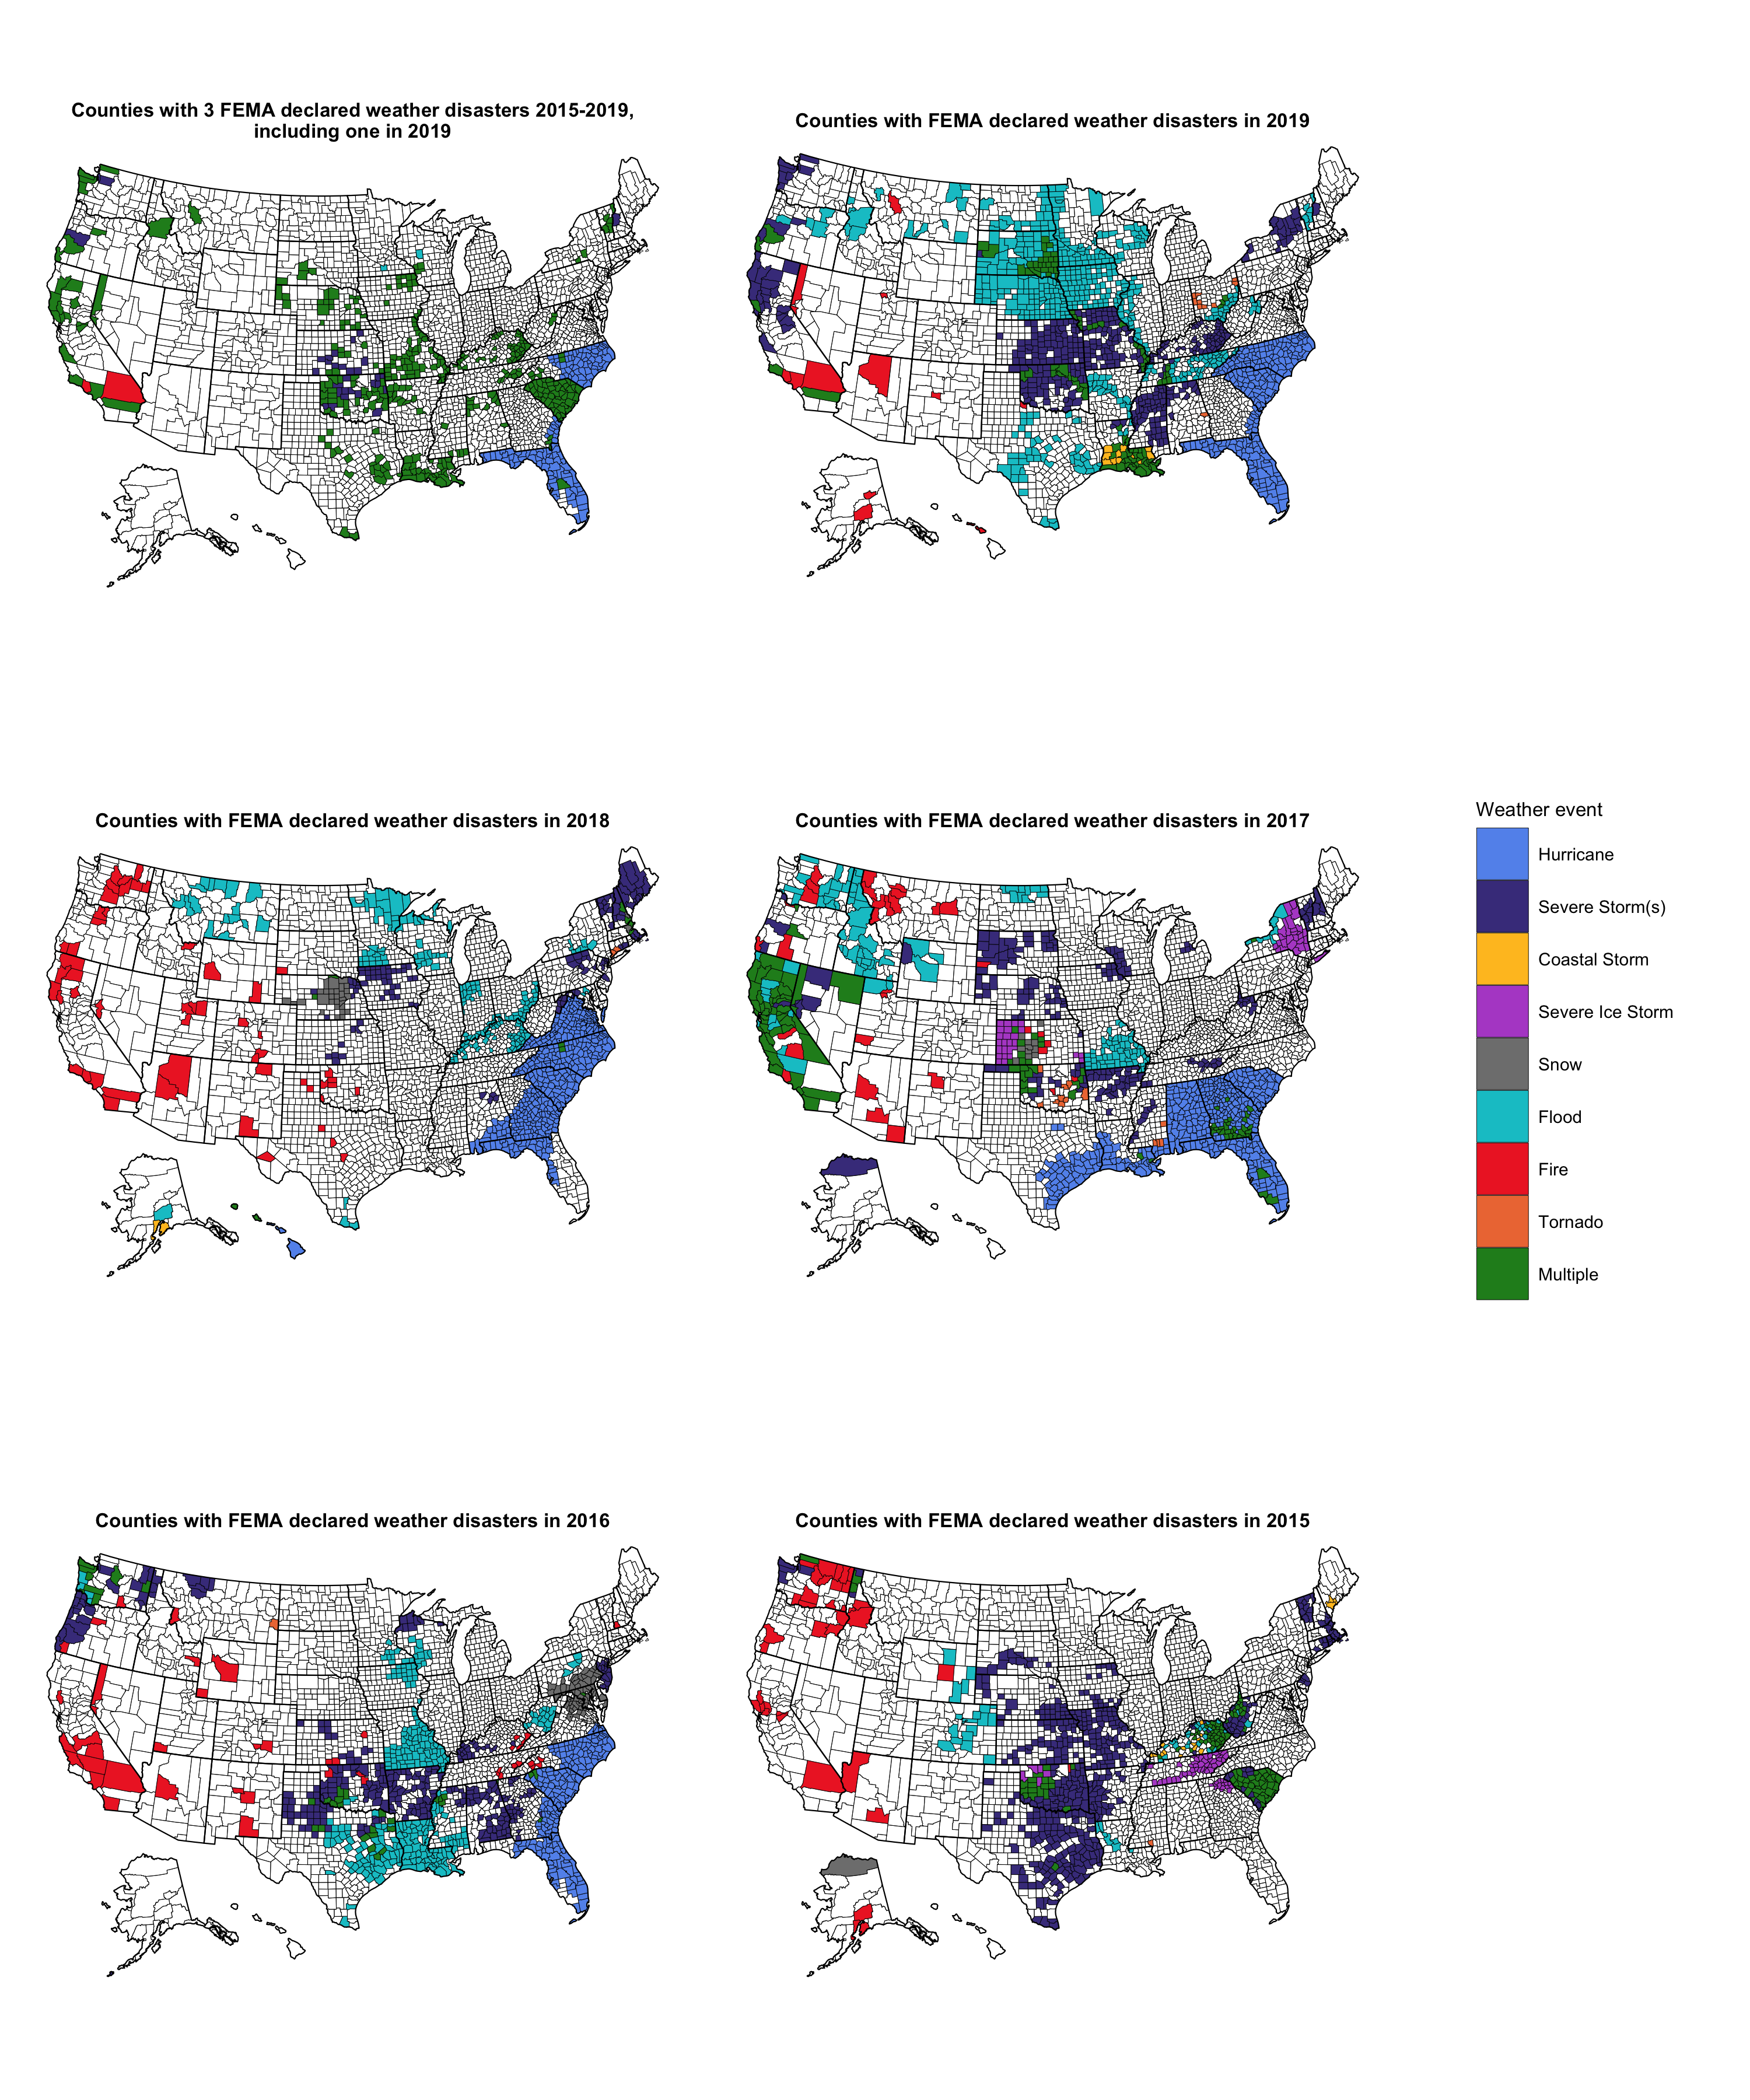
\includegraphics[scale=0.175]{images/fema_events_maps_combined.png}
\caption{Upper left: counties with FEMA declared disasters that are flagged as "affected by severe weather" in this analysis. The rest of the plots show all FEMA declared weather disasters from 2015-2019. Larger plots are available in code directory.}
\end{figure}


\section{Analysis}
Three different approaches were used to try to understand the impact of these extreme weather events on the county-level climate change beliefs: linear regression, a county matching procedure between counties that did and did not experience extreme weather as defined in this report, and hypothesis testing of average beliefs between clusters of counties. Before attempting any of these, the relationship between each covariate and the response variable (belief in climate change) was explored to determine a smaller subset of variables to use in the analysis. 

\subsection{Covariate selection}
Within the Census-provided covariates, median age, median income, proportion of non-white population, proportion of Asian population, and proportion of Hispanic population were identified as appearing most predictive of climate change belief. Other variables for race and ethnicity proportions appeared to be somewhat predictive, but were left out in an attempt to allow for better county-to-county matching on the most predictive variables. The 2020 election data includes proportions of votes to Green, Libertarian, and "Other" candidates in addition to the major two parties. Shares of votes to these third party candidates were initially expected to be somewhat predictive of climate change belief, in particular the share of Green party votes, but none where anywhere close to as strong as the share of votes to Joe Biden or Donald Trump. Therefore the approaches listed above only considered the share of votes to the Democratic candidate (with share of votes to the Republican candidate being almost perfectly negatively correlated with a correlation value of -0.999, as one would expect). To quickly test the hypothesis that political leaning alone, a simple one-way ANOVA was performed on average belief in climate change between counties that voted majority Democrat and counties that voted majority Republican. The test is visualized in the boxplot below, the resulting p-value of $<0.01$ strongly rejecting the null that political affiliate has no impact on climate change belief.

\begin{figure}[H]
\centering
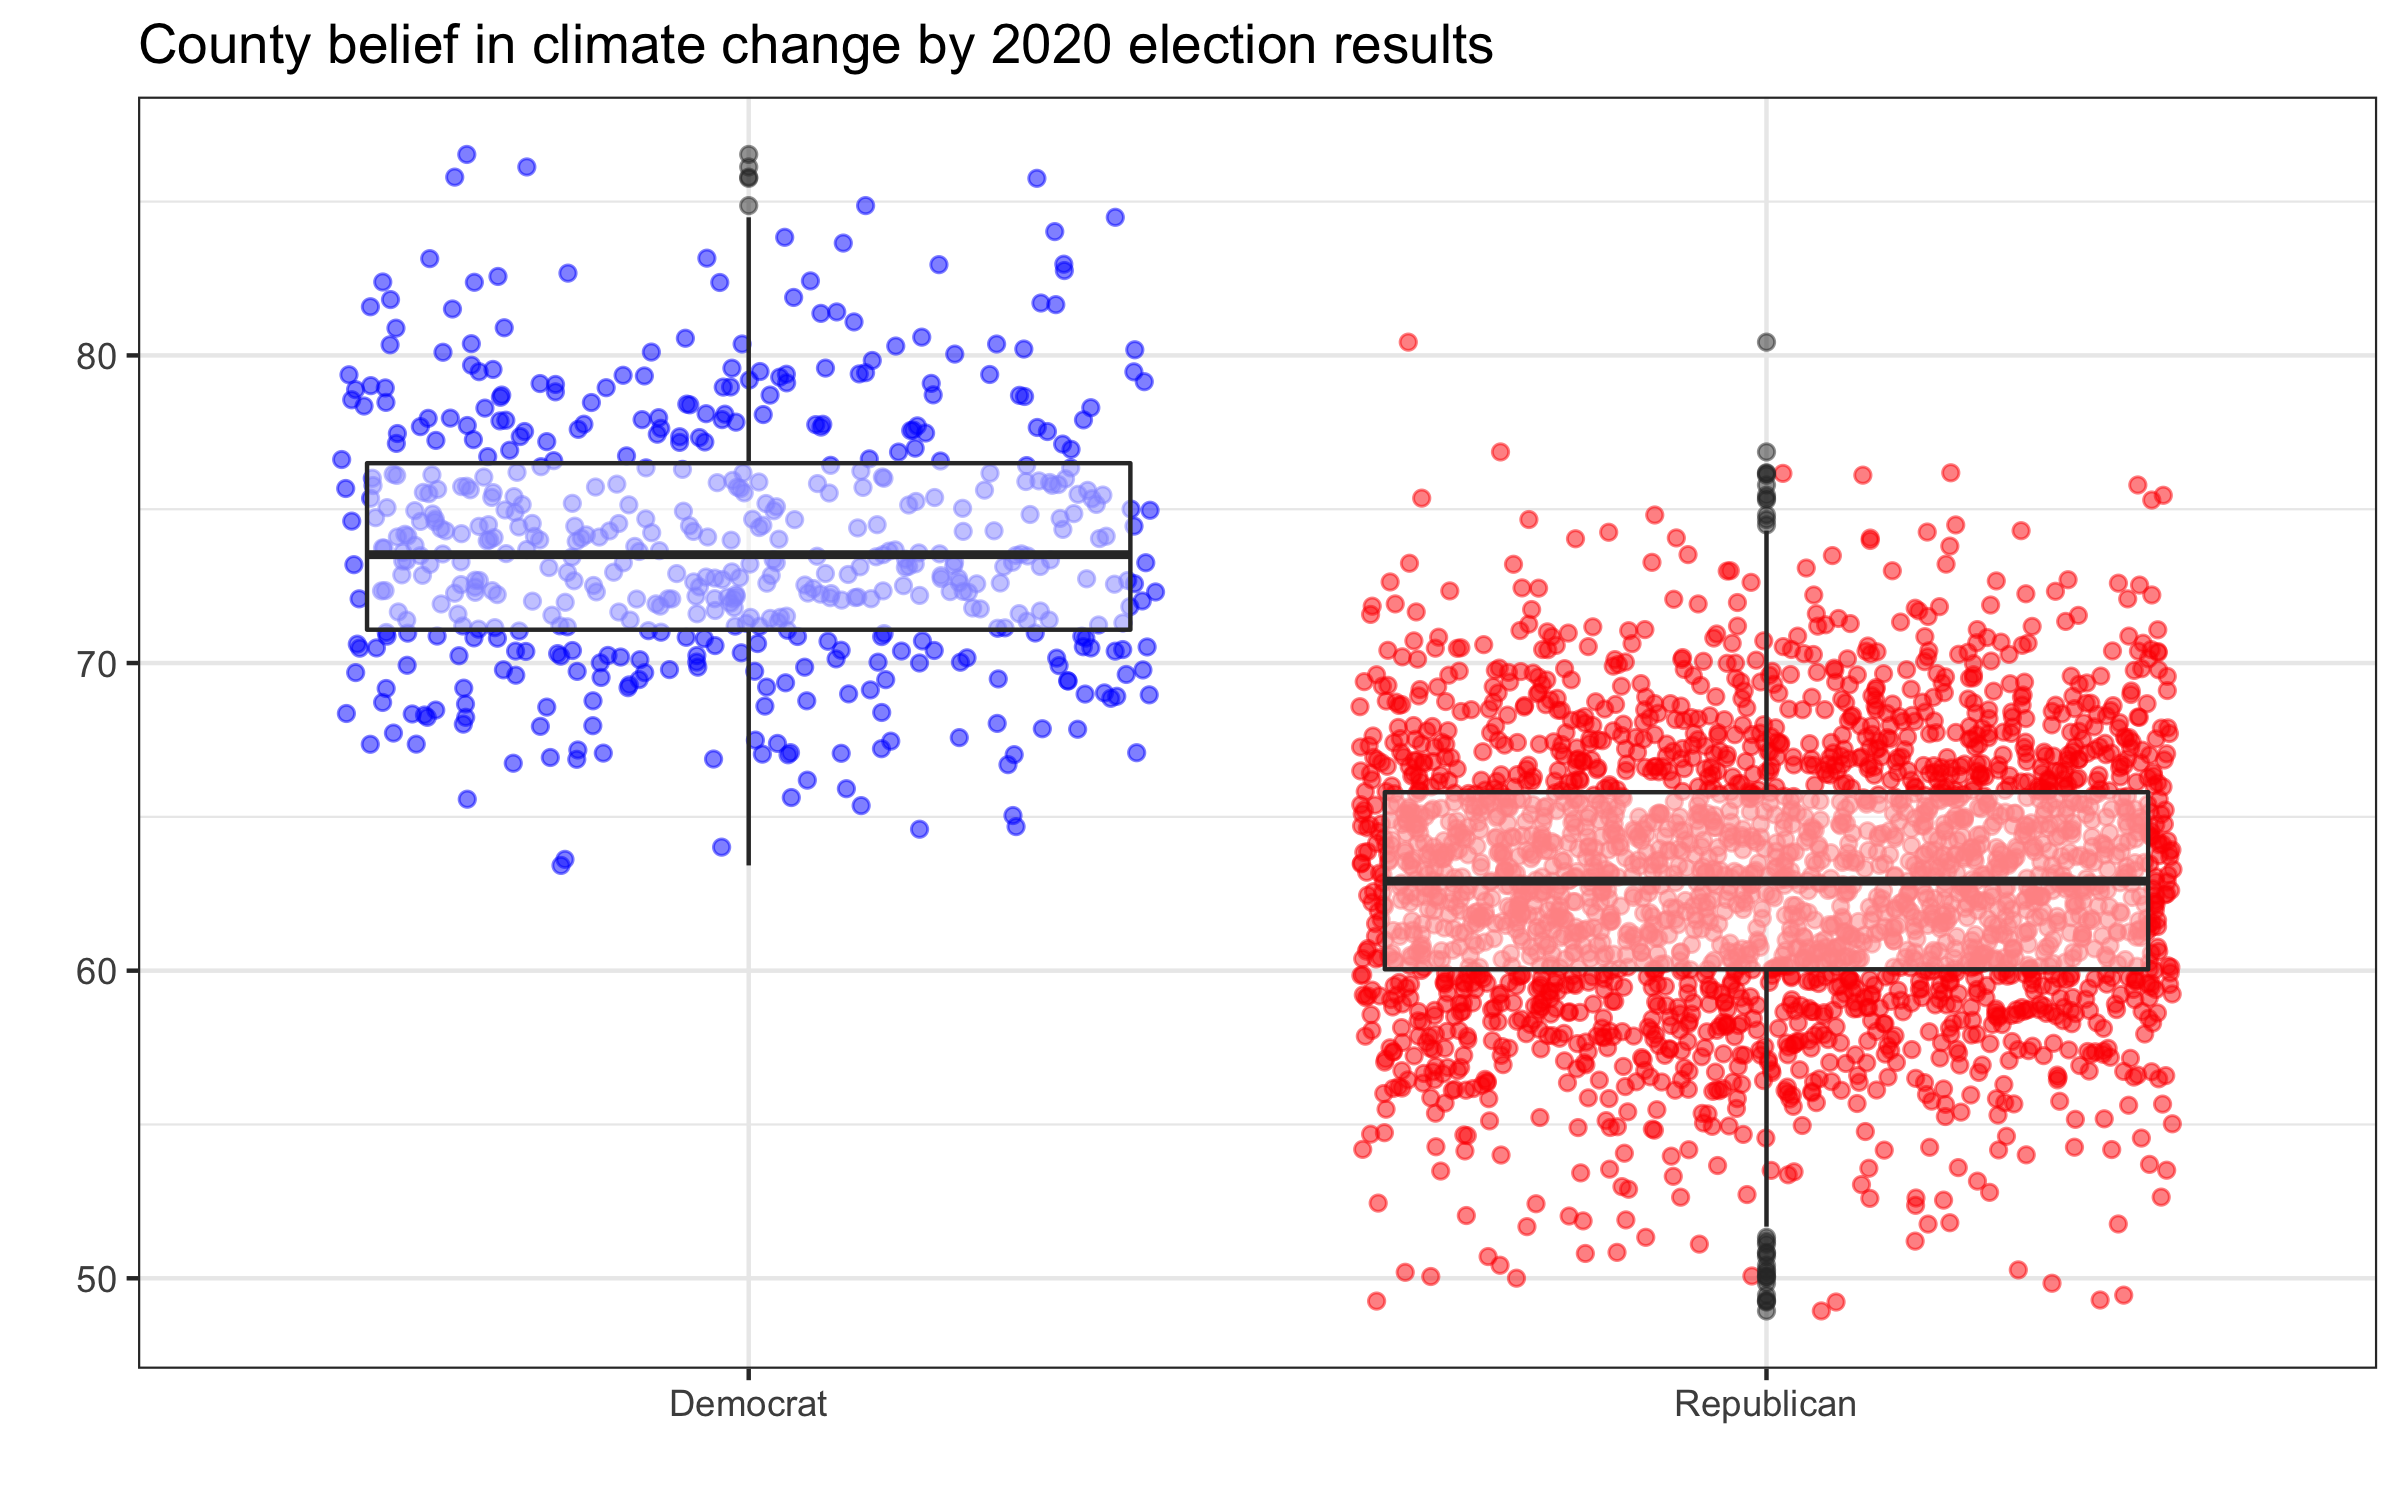
\includegraphics[scale=0.2]{images/election_party_anova.png}
\caption{On average, counties that voted majority Democrat in the 2020 general election are estimated to have about 74\% of county population believing in climate change, while counties that voted majority Republican are estimated to have about 63\% of county population believing in climate change. This is a difference of 11\%, and the resulting t-statistic is -54.21.}
\end{figure}

The data meets the requirements for ANOVA testing. The distribution of climate change beliefs is approximately Normal, these responses are assumed to be independent, and the variance between groups is approximately equal (the standard deviation of the response for Republican-leaning counties is approximately 4.32, while the standard deviation of the response for Democratic-leaning counties is approximately 4.12). 

\subsection{Regression model, matching, and clustering approaches}
Beginning with the simpler approach, the identified covariate were used in a linear regression along with the discussed extreme weather flag for predicting county climate change belief. Square-root transforms were applied to the population proportion variables rather than the log transform, as multiple counties had population proportions of 0 for some groups. The log transform was applied to the median income covariate. Model diagnostic tests passed, as the residuals appeared to be close to Normal and residual variance looked fairly equal across fitted values. This procedure was repeated using an extreme weather flag specifically for counties that experienced hurricanes, using the same logic of only flagging a county if it experienced a hurricane in 2019 in addition to two others since 2015. Hurricanes specifically were chosen for this additional analysis because they are the type of event that affected the most counties the most often. 

For the second approach towards understanding the relationship between extreme weather events and climate change belief, the R package MatchIt was used. This package is developed for causal inference applications, and "performs pairing, subset selection, and subclassification with the aim of creating treatment and control groups balanced on included covariates", as stated in its documentation. This analysis does not consist of a proper causal inference framework, for reasons including the lack of randomization between "treatment" of experiencing an extreme weather event, and the fact that belief estimates are obtained only at the county level rather than the individual level. However, the package and ideas behind comparing "treatment" and "control" group responses are still helpful for the goals of this report. Using MatchIt, counties that were flagged as experiencing extreme weather were matched to counties that did not, but were as similar as possible to the first county with respect to the selected covariates. In particular, the "optimal" matching method was used, which minimizes the sum of absolute pairwise distances in the matched sample. This lowers the probability of extreme within-pair distances with respect to covariates. Figure 4 shows the effects of matching on the standardized mean difference of the covariates of counties with and without the extreme weather flag.

\begin{figure}[H]
\centering
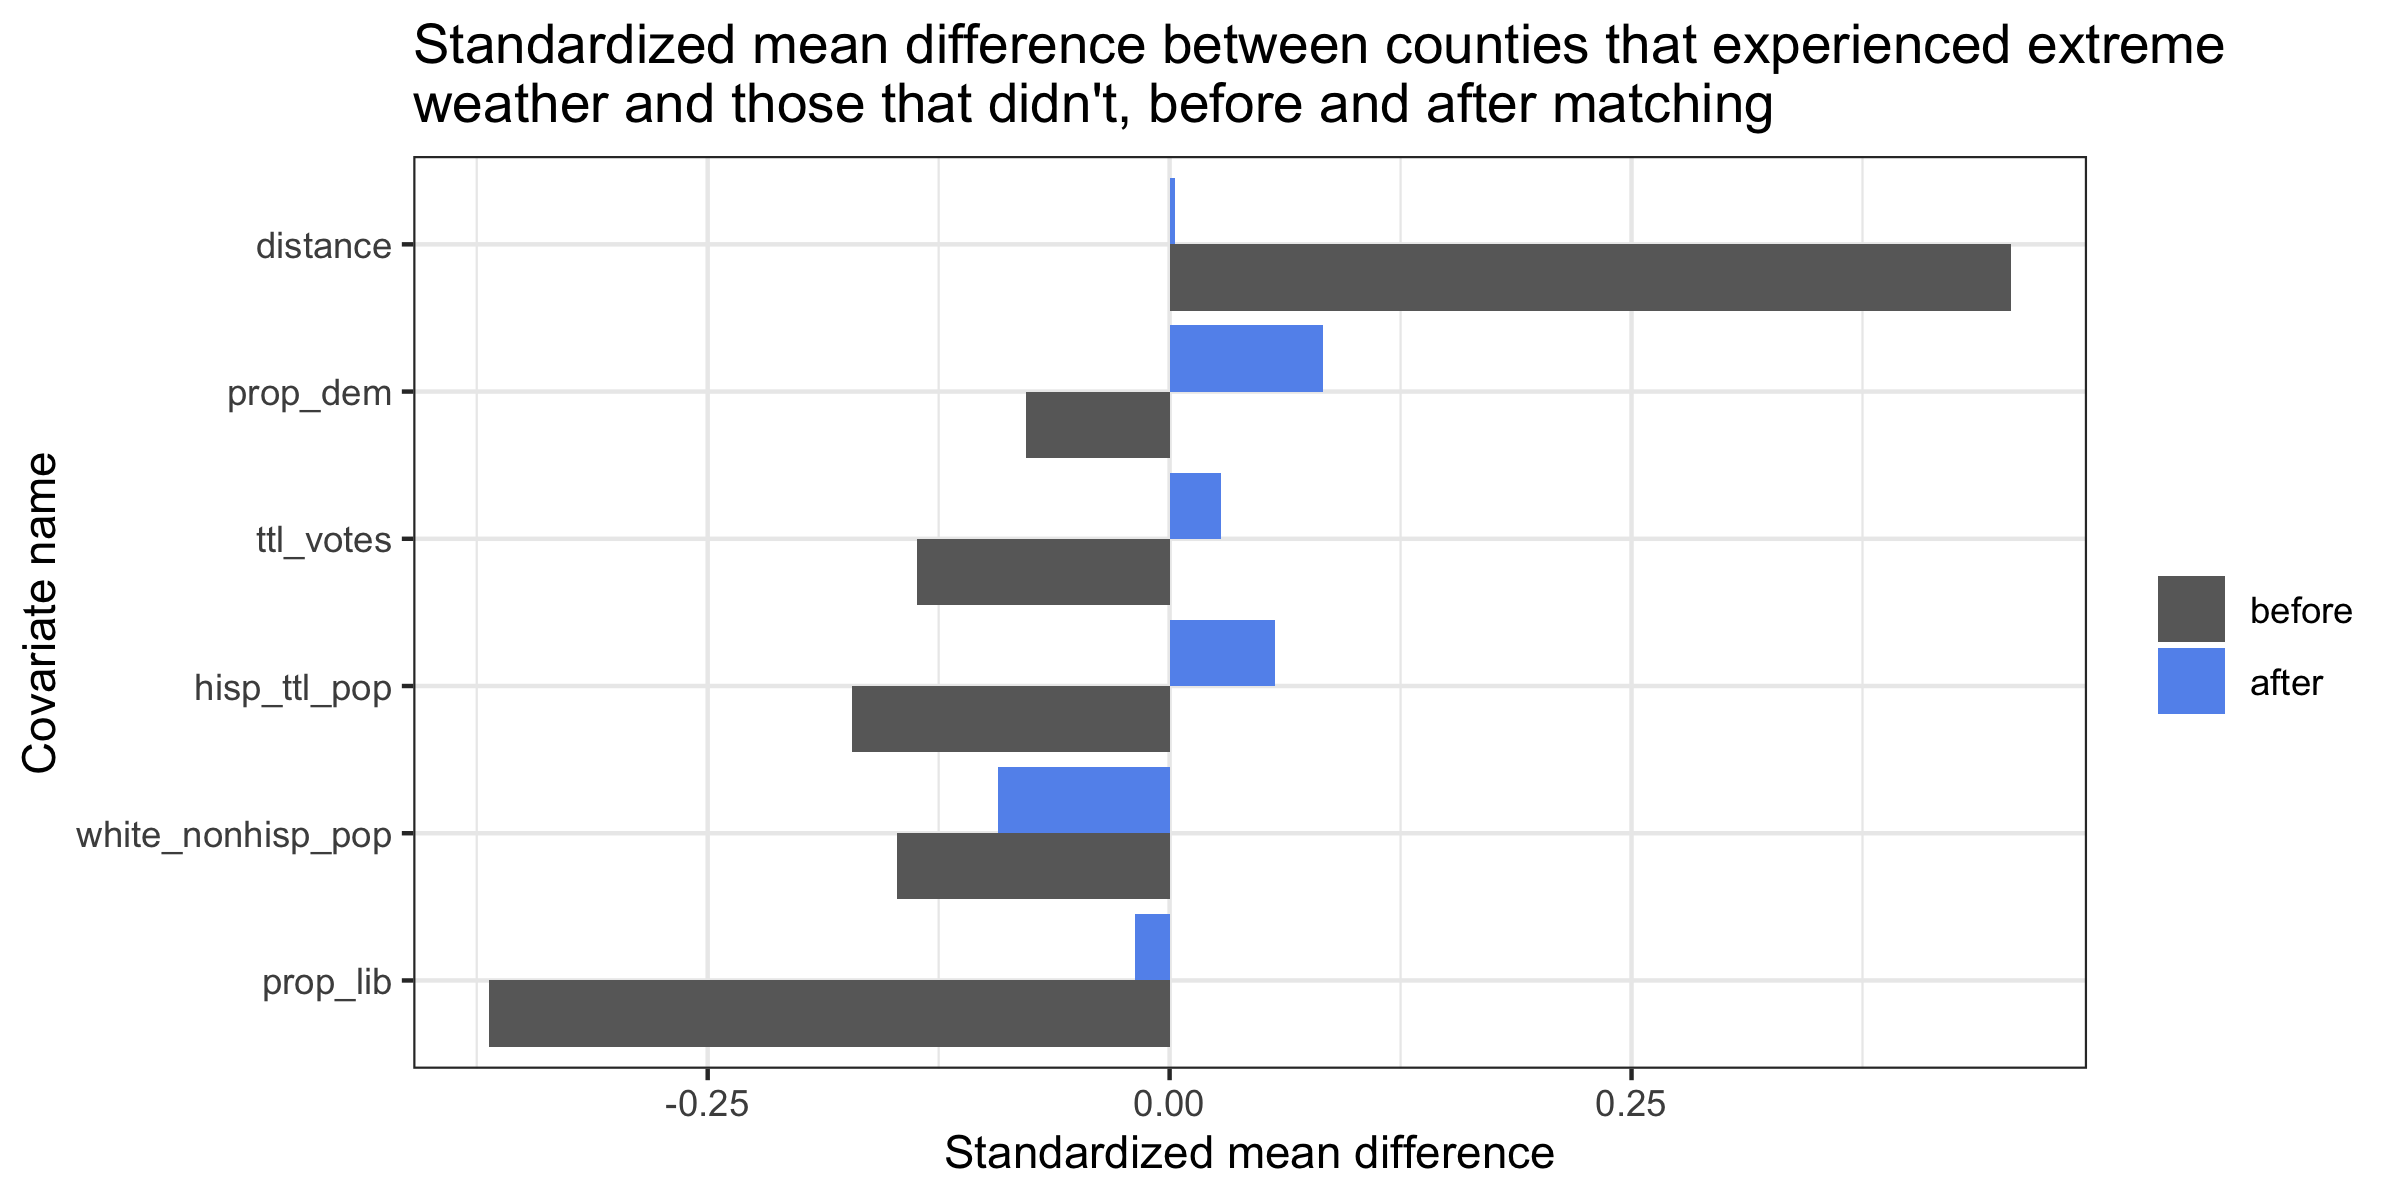
\includegraphics[scale = 0.2]{images/matching_balance_plot.png}
\caption{This figure shows that matching via MatchIt was able to reduce the standardized mean difference between all covariates but the median age, whose standardized mean difference actually increased.}
\end{figure}

Once counties were matched, the difference in climate change belief was calculated between each pair. The average of these differences serves as a metric for how experiencing extreme weather affects the probability of otherwise similar counties' beliefs in climate change.

Finally, a clustering approach was applied to the data to see how counties similar to each other in more granular terms compared with respect to climate change belief. To minimize the number of clusters, four covariates found to be most predictive in the initial exploratory analysis - political leaning, median age, proportion of population identifying as white, and median income - were discretized into two categories each. Median age was divided into "Young Adults" and "Adults", using age 35 as the threshold, which seems to be a common cut-off for studies utilizing age. Counties were categorized as having a "high" proportion of white residents if they had a proportion above the national proportion (which the Census Bureau reported to be 76.3\% in 2019),  and "low" otherwise. Similarly, counties were categorized as having a "high" median income if the county median income exceeded the national median income of \$62,843 (as reported by the Census in 2019), and "low" otherwise. Though median age, income, and demographics vary quite a lot from state to state, national thresholds are used rather than state thresholds because counties are ultimately compared from between different states, so it seems more reasonable to categorize counties uniformly. Finally, counties were classified as either "red" or "blue" depending on if the majority of the 2020 general election vote went to Biden or Trump. The resulting 16 clusters were then split further into pairs based on whether or not they had experienced extreme weather.

To maintain the ANOVA assumption of equal variances, pairs were removed from the cluster analysis if the maximum standard deviation of the pair exceeded the minimum standard deviation by 2 or more. Pairs were also removed if one or both clusters had less than 20 counties attributed to it. Only four pairs of clusters survived these requirements, and Q-Q plots were checked for each of these clusters to ensure that the responses of each were roughly Normal. Finally, ANOVA was performed on each pair, testing the null hypothesis that the mean climate change belief of each cluster (differing only by the experience of extreme weather) was the same. To account for multiple testing, the Benjamini-Hochberg correction was applied to control for false detection rate. This less conservative test controlling the FDR was used rather than a correction such as Bonferroni because stakes are low if there is a false positive, so it seems appropriate rather than controlling for family-wise error.

\section{Results}
The summary of the linear regression analysis is displayed in Figure 5, where we can see that the coefficient of the flag for witnessing extreme weather is small, positive, and significant to the $\alpha = 0.01$ level. This value indicates that counties that witnessed an extreme weather event are likely to have a slightly higher belief in climate change by about 0.41 (in percentage, not proportion). As expected, counties with a higher proportion of the 2020 election vote going to Joe Biden are much more likely to believe in climate change. Interestingly, counties with an older median age are predicted to also be slightly more likely to believe in climate change, which may be surprising as a common perception is that younger generations care much more about the environment. Counties with less diverse populations with respect to Asian and Hispanic individuals are predicted to be less likely to believe in climate change. 

\begin{figure}[H]
\centering
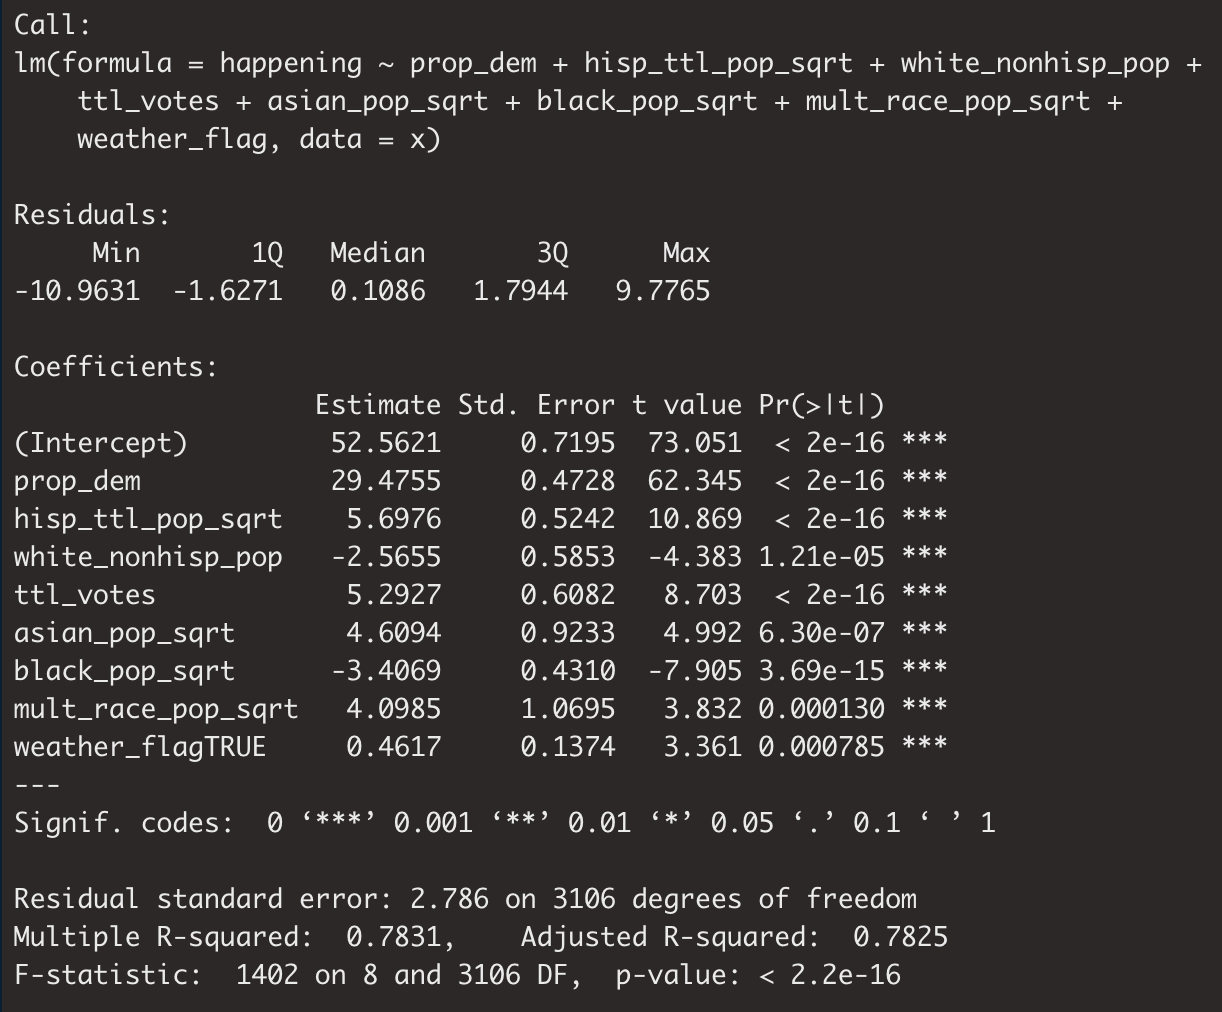
\includegraphics[scale=0.4]{images/regression_summary.png}
\caption{Summary of linear regression model predicting county climate change belief.}
\end{figure}

A repeated analysis looking just at counties that experienced hurricanes in particular tells a very similar story but with a larger and more significant coefficient for experiencing the extreme weather: an additive increase of 1.02\% is predicted for those counties that experienced hurricanes in 2019 as well as twice more since 2015. 

The metric calculated from the matching process described above falls in a similar range, with the average difference in county belief between matched pairs calculated to be 0.78\%, indicating again that experiencing an extreme weather event may increase belief in climate change slightly. The repeated analysis for experiencing hurricanes specifically resulted in a value of 1.29\%, mirroring the increase seen in the regression analysis between comparing counties that experienced any weather and counties that specifically experiences hurricanes.

The clustering analysis had less conclusive results, which are shown in Table 1 below. For low income, older, whiter, and more Republican counties, the test found that experiencing a weather event had a small but significant negative effect on climate change beliefs. Alternatively, in counties that are lower income, older, more Republican, but with smaller white populations, the test found that experiencing a weather event had a small but significant positive effect on climate change beliefs. If this analysis were at a finer granularity of population (such as towns, congressional districts, etc), more clusters may have a larger amount of samples and thus more interesting heterogeneous results. However, in this case the number of counties limits the extent to which this cluster analysis is very meaningful. The small amount of counties that make it into each cluster also meant that the analogous hurricane analysis was not possible for this approach.  

\begin{center}
\begin{table}
\begin{tabular}{| c | c | c | c | c | c | c | c | c | c ||}
\hline
Pair & Political & Median Age & White Pop. & Median Income & $n$ & Mean Diff. & p-value & BH p-value \\ [0.5ex]
\hline
\hline
1 & Red & Adult & High & Low & 1424, 265 & -0.8739 & 0.0016 & 0.0065 \\
\hline
2 & Red & Adult & Low & Low & 285, 107 & 1.1322 & 0.0067 & 0.0202 \\
\hline
3 & Blue & Adult & Low & Low & 111, 38 & 0.8758 & 0.2284 & 0.2284 \\
\hline
4 & Red & Adult & High & High & 276, 28 & 1.1853 & 0.1638 & 0.2284 \\
\hline
\end{tabular}
\caption{Results of clustering analysis. Values for $n$ are listed in the order: did not experience extreme weather, did experience extreme weather. Positive mean difference values indicate that counties that did experience extreme weather had higher average belief in climate change than those those that did not.}
\end{table}
\end{center}


\section{Conclusion}
The results of the multiple approaches explored in this analysis imply that recently experiencing an extreme weather event, in places where these types of events have become more common over the past 5 years, may increase the likelihood of the average individual believing that climate change exists. In particular, experiencing hurricanes seems to have a potentially larger positive effect. However, these effects may be heterogeneous between subsets of the population with different racial, socioeconomic, and political features, though this analysis is limited in its exploration of differences between such subsets via the cluster analysis described here. Though more variations of clusters could be formed through unsupervised learning or using different thresholds to separate the population by differently discretized covariates, this approach may sacrifice interpretability. As one may expect, the linear regression approach demonstrated how strongly political leaning influences climate change belief, indicating that even if more convincing effects of extreme weather were found, they would still likely be eclipsed by the effect of political polarization. 

\newpage
\section{References}

\subsection{Contextualizing the problem of climate change and climate change communication}
\begin{itemize}
	\item Guardian article about current climate change crisis: \url{https://www.theguardian.com/environment/ng-interactive/2021/oct/14/climate-change-happening-now-stats-graphs-maps-cop26}
	\item Organization for climate change communication: \url{https://climate-xchange.org/communicating-the-climate-crisis/}
	\item Yale Climate Communication Group: \url{https://climatecommunication.yale.edu/}
\end{itemize}

\subsection{Data sources}
\begin{itemize}
	\item Climate change opinion data: \url{https://climatecommunication.yale.edu/visualizations-data/ycom-us/}
	\item Election data: MIT Election Data and Science Lab, 2018, "County Presidential Election Returns 2000-2020", \url{https://doi.org/10.7910/DVN/VOQCHQ}, Harvard Dataverse, V9, UNF:6:qSwUYo7FKxI6vd/3Xev2Ng== [fileUNF]
	\item Census Bureau ACS Estimates: \url{https://www.census.gov/programs-surveys/acs/data.html}
	\item FEMA disaster data: \url{https://www.fema.gov/about/openfema/data-sets#disaster}
\end{itemize}

\subsection{Analysis documentation}
\begin{itemize}
	\item MatchIt package: \url{https://kosukeimai.github.io/MatchIt/reference/method_optimal.html}
	\item TidyCensus package: \url{https://cran.r-project.org/web/packages/tidycensus/tidycensus.pdf}
\end{itemize}



\end{document}